
\documentclass{beamer}
\usepackage[T1]{fontenc}
\usepackage[polish]{babel}
\usepackage[utf8]{inputenc}
\usepackage{array}
\usepackage{url}
\usetheme{Goettingen}
\setbeamertemplate{frametitle continuation}{}
\titlegraphic{
\includegraphics[width=2cm]{../perebor_5.jpg}}        
\title{AI jako program komputerowy}
\author{Robert Trypuz}
\institute{AI po lekcjach}
\date{2024-03-09}

\begin{document}
\frame{\titlepage}
  

\section{INTRO}

\begin{frame}[fragile]
\frametitle{Wprowadzenie}
 \begin{itemize}
\item Myśląc i dyskutując o sztucznej inteligencji, często zapominamy, że jest ona w istocie programem komputerowym.
\item Czym są programy komputerowe i które z nich możemy nazwać sztuczną inteligencją (AI)? 

                    \begin{figure}[h]
                        \centering
                        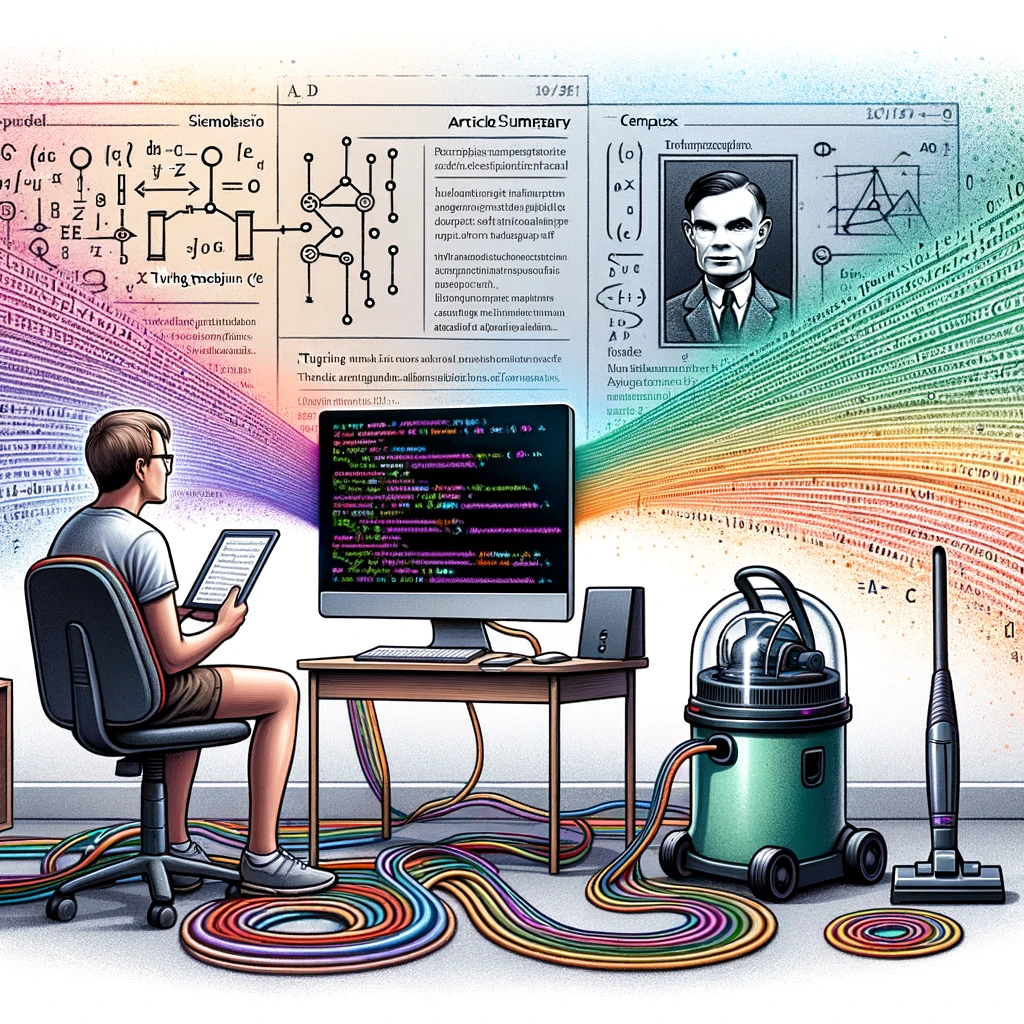
\includegraphics[width=0.5\textwidth]{../../img/o_komputerze.png}
                    \end{figure}                    
                    \end{itemize}

\end{frame}

\section{I. O komputerze}

\begin{frame}[fragile]
\frametitle{Maszyna Turinga}
 \begin{itemize}
\item W 1936 roku \textbf{Alan Turing} stworzył teoretyczny model komputera (nazwany później Maszyną Turinga).

                    \begin{figure}[h]
                        \centering
                        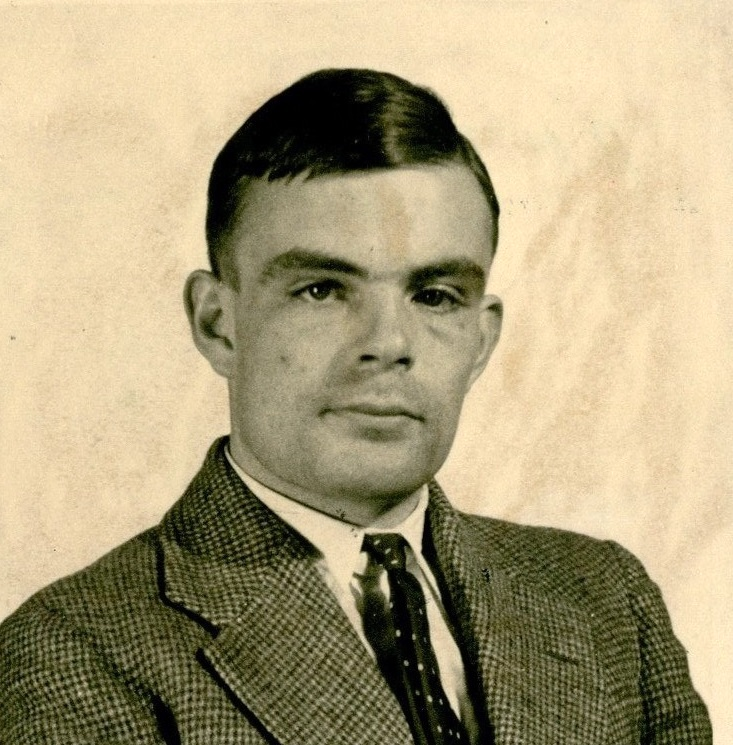
\includegraphics[width=0.5\textwidth]{../../img/Alan_Turing_1912-1954_in_1936_at_Princeton_University.jpg}
                    \end{figure}                    
                    \item Pozwala on nam ocenić: 
	\begin{itemize}
	\item jakie problemy komputer może rozwiązać
	\item jak złożony jest dany problem z perspektywy komputera, tzn. jak wiele pamięci i ile operacji komputer będzie potrzebował na jego rozwiązanie.
	\end{itemize}
\end{itemize}
\end{frame}

\begin{frame}[fragile]
\frametitle{Uniwersalność komputera}
\begin{itemize}
\item Jedną z podstawowych zalet komputera jest jego \textbf{uniwersalność}.
	\begin{itemize}
	\item inne urządzenia domowe jak na przykład odkurzacz mają ściśle określone przeznaczenie i wąski zakres czynności jaki możemy za ich pomocą wykonać
	\item komputer wykazuje zdolność do realizacji znacząco szerszej gamy zadań.
	\end{itemize}
\item Ta uniwersalność ma jednak swoją cenę: musimy komputerowi odpowiednio zakomunikować co i jak ma robić w języku, który jest on w stanie "zrozumieć". 
\end{itemize}

\end{frame}

\section{II. Komunikacja i programowanie}

\begin{frame}[fragile]
\frametitle{Programowanie to sposób komunikacji człowieka z komputerem}
 \begin{itemize}
\item \textbf{Programowanie} to sposób komunikacji człowieka z komputerem, którego celem jest rozwiązanie jakiegoś problemu.
\item Problemy stawiane przed komputerem mogą być 
	\begin{itemize}
	\item proste, np. obliczenie wyniku mnożenie dwóch liczb
	\item bardziej złożone, jak napisanie streszczenia kilkustronicowego artykułu.
	\end{itemize}
\item Skoro programowanie to sposób komunikacji człowieka z komputerem, to takiego człowieka, który potrafi skutecznie taką komunikację prowadzić nazwiemy \textbf{programist(k)ą}. 
\item Co ciekawe, programist(k)a komunikuje się z komputerem w podobny sposób jak ludzie komunikują się między sobą - używa języka. 
\end{itemize}
\end{frame}

\begin{frame}[fragile]
\frametitle{Programowanie to sposób komunikacji człowieka z komputerem}

                    \begin{figure}[h]
                        \centering
                        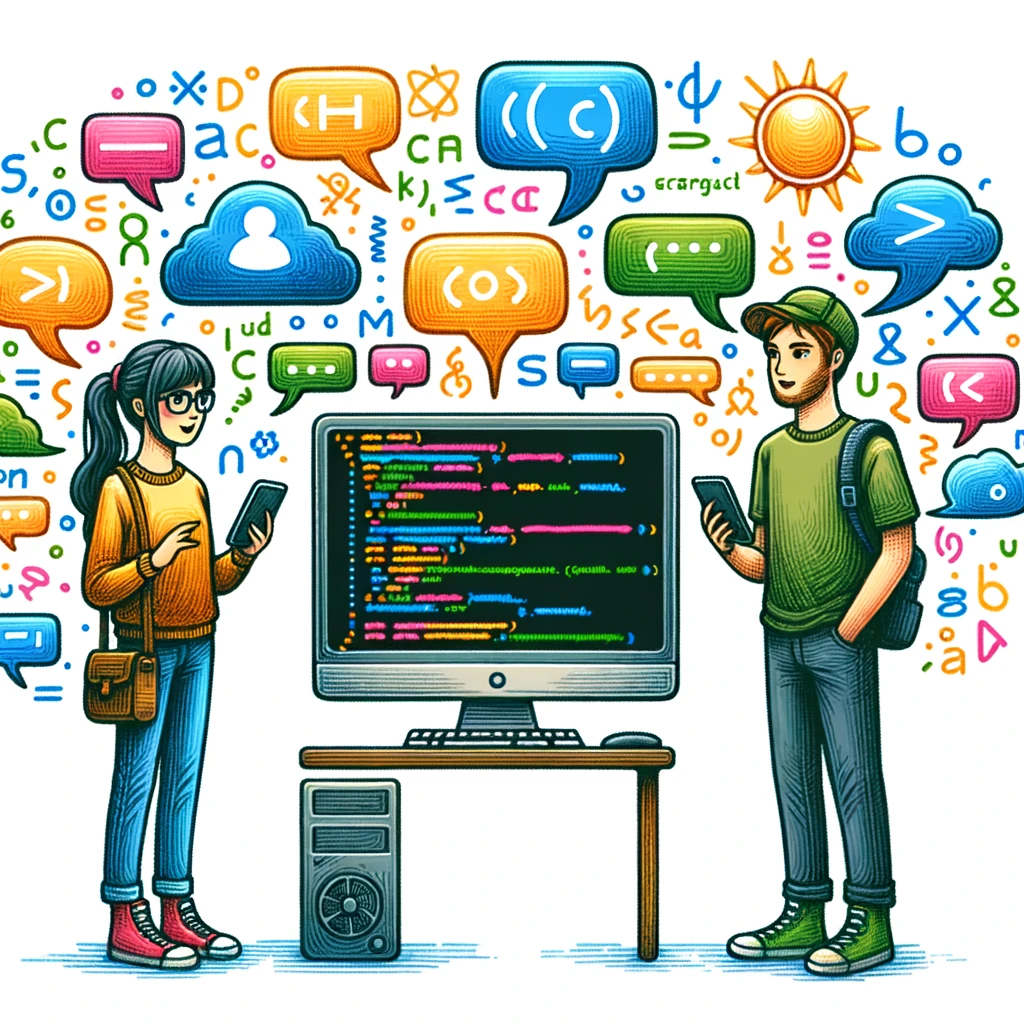
\includegraphics[width=0.5\textwidth]{../../img/komunikacja4.png}
                    \end{figure}                    

\end{frame}

\begin{frame}[fragile]
\frametitle{Komunikacja}
\begin{itemize}
\item Komunikujemy się wymieniając komunikaty.
	\begin{itemize}
	\item Każdy komunikat składa się z słów ułożonych w pewnym porządku, który to porządek definiuje gramatyka języka, którym się posługujemy.
	\item Komunikat jako całość ma też swoją treść (czyli sens), który komunikujący chce odbiorcy tego komunikatu przekazać.
	\end{itemize}
\item Gdy komunikat jest niepoprawny gramatycznie, często nie możemy go zrozumieć. 
\item Tak samo jest, gdy komunikat, choć gramatycznie poprawny, zawiera wyrażenia, których znaczenia (czyli sensu) nie znamy. 
	\begin{itemize}
	\item W obu przypadkach mówimy: „To jest bez sensu!”.
	\end{itemize}
\item Tak więc sprawne używanie języka w komunikacji, zarówno tej międzyludzkiej, jak i między człowiekiem a komputerem, wymaga formułowania komunikatów w języku zrozumiałym dla odbiorcy i to w sposób gramatycznie poprawny, dobierając odpowiednie wyrażenia tak, aby całość komunikatu była sensowna. 
\end{itemize}

\end{frame}

\section{III. Języki programowania i program komputerowy}

\begin{frame}[fragile]
\frametitle{Języki programowania}
 \begin{itemize}
\item Tak jak jest wiele języków, którymi ludzie komunikują się między sobą, tak też jest wiele języków służących do komunikacji z komputerem, np. Python czy Java, żeby wymienić tylko dwa najpopularniejsze.
\item Nazywamy je \textbf{językami programowania}. 

                    \begin{figure}[h]
                        \centering
                        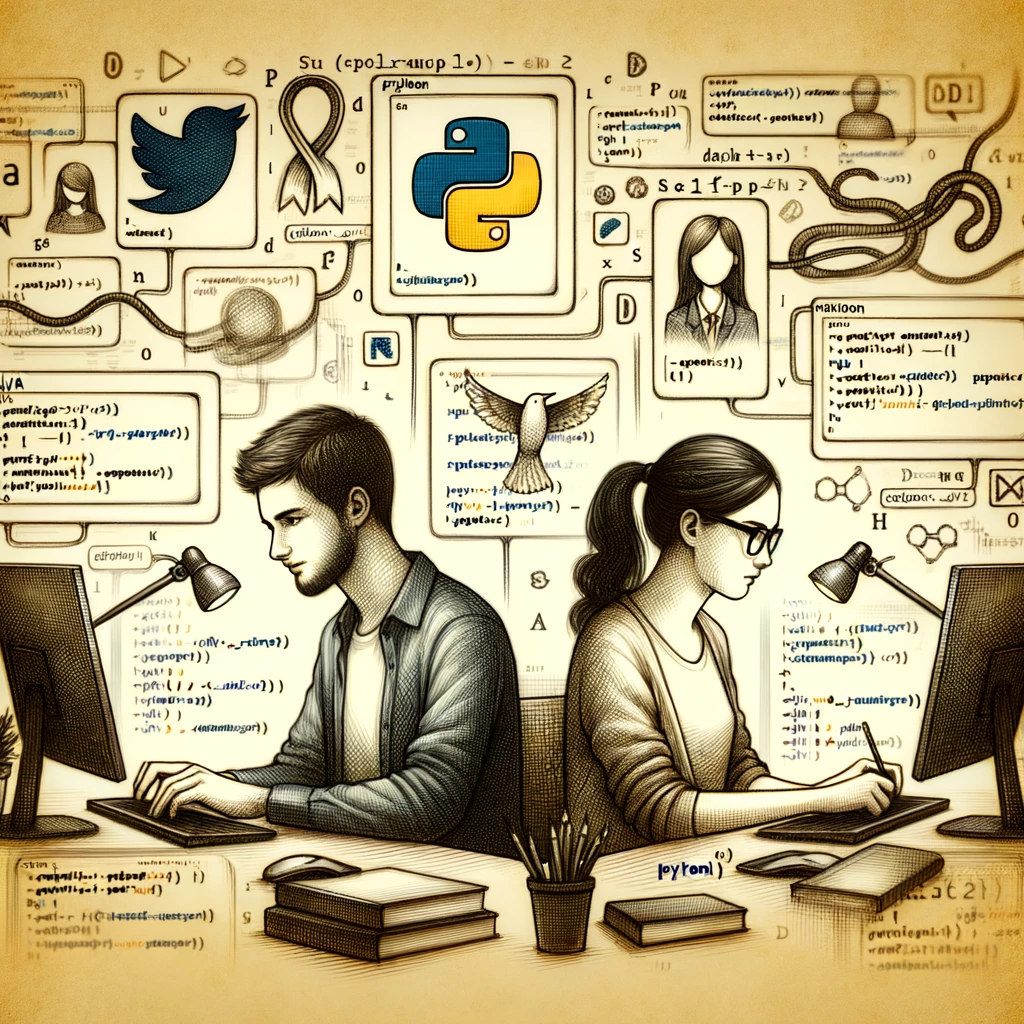
\includegraphics[width=0.5\textwidth]{../../img/program_komputerowy3.png}
                    \end{figure}                    
                    \end{itemize}
\end{frame}

\begin{frame}[fragile]
\frametitle{Języki programowania}
\begin{itemize}
\item Język programowania, jak każdy język
	\begin{itemize}
	\item ma swój system znaków
	\item swoją gramatykę
	\item reguły definiujące znaczenie/sens wyrażeń (czyli jaki efekt osiągniesz używając tego czy innego wyrażenia).
	\end{itemize}
\item Jeśli zostaniesz programist(k)ą, komunikując się z komputerem (np. za pomocą Pythona czy Javy), będziesz wysyłał(a) komputerowi komunikaty instruujące go jakie kroki kolejno powinien on wykonać. 
	\begin{itemize}
	\item To jest tak, jakbyś pisząc program komputerowy wydawał(a) komputerowi rozkazy: zrób to, a potem tamto, a następnie to, itd.
	\end{itemize}
\end{itemize}
\end{frame}

\begin{frame}[fragile]
\frametitle{Programowanie i program komputerowy}
\begin{itemize}
\item Zatem \textbf{programowanie} to wprowadzanie instrukcji, które mówią komputerowi, co ma robić krok po kroku, zgodnie z intencją programisty lub programistki.
\item Zbiór takich instrukcji nazywa się \textbf{programem komputerowym}. 
\item I choć instrukcje zawarte w programie komputerowym potrafią być bardzo złożone, a profesjonalne oprogramowanie może składać się nawet z milionów linii kodu, to zawsze kod ten można rozłożyć na prostsze instrukcje postaci: 
	\begin{itemize}
	\item Zrób to!
	\item Jeżeli jest taka a tak, zrób to, w przeciwnym przypadku zrób co innego!
	\item Wykonaj to 10 razy!
	\end{itemize}
\item Jeśli zdecydujesz się na naukę programowania, to zapewne zaczniesz od nauczenia się tych prostych instrukcji i sukcesywnie będziesz uczyć się składania ich w większe programy komputerowe. 
\item \textbf{Pamiętaj!} Nie ma zasadniczej różnicy w uczeniu się języka obcego jak angielski czy włoski, a uczeniem się języka programowania Python, czy Java. 
\end{itemize}

\end{frame}

\section{IV. Inteligentne programy komputerowe}

\begin{frame}[fragile]
\frametitle{Inteligencja}
 \begin{itemize}
\item Czy każdy program komputerowy jest sztuczną inteligencją?
\item Kiedy nazwiemy program komputerowy “inteligentnym”? 

                    \begin{figure}[h]
                        \centering
                        
\includegraphics[width=0.5\textwidth]{../../img/inteligentne_programy.png}
                    \end{figure}                    
                    \end{itemize}
\end{frame}

\begin{frame}[fragile]
\frametitle{Inteligencja}
\begin{itemize}
\item Zanim odpowiemy na te pytania poświęćmy chwilę samej “inteligencji”.
\item Nie ma konsensusu wśród uczonych czym dokładnie jest inteligencja. 
\item Sympatyzuję z teorią inteligencji wielorakiej Howarda Gardnera zgodnie z którą \textbf{inteligencja} rozumiana jest jako zestaw różnych procesów myślowych, które umożliwiają przetwarzanie informacji, rozwiązywanie problemów, podejmowanie decyzji, rozumienie emocji, tworzenie sztuki i wykonywanie przeróżnych skomplikowanych działań. 
\item \textbf{Nie ma więc jednej inteligencji, jest ich wiele.} 
\end{itemize}
\end{frame}

\begin{frame}[fragile]
\frametitle{Inteligencja}
\begin{itemize}
\item Tak też przejawami procesów myślowych świadczących o tym, że posiadamy w różnym stopniu wiele inteligencji będą:
	\begin{itemize}
	\item kierowanie autem
	\item rozmowa z przyjacielem
	\item właściwe odczytanie emocji z wyrazu twarzy partnerki czy partnera
	\item stworzenie szkicu Archikatedry Lubelskiej
	\item napisanie streszczenia artykułu
	\item podjęcie decyzji odnośnie kierunku studiów poprzedzone wielogodzinnymi rozważaniami “za i przeciw”
	\item zrobienie ollie na deskorolce
	\item czy w końcu odnalezienie ulubionego sklepu z butami w dużej galerii handlowej.
	\end{itemize}
\end{itemize}
\end{frame}

\begin{frame}[fragile]
\frametitle{Inteligentne programy komputerowe}
\begin{itemize}
\item \textbf{Programy komputerowe nazwiemy inteligentnymi}, gdy będą automatyzować procesy myślowe standardowo wykonywane przez ludzi.
\item To znaczy, gdy uda nam się napisać program komputerowy, który samodzielnie pokieruje autem lub napisze streszczenie artykułu lub przeprowadzi poprawne rozumowanie lub rozpozna, czy recenzja filmu jest pozytywna, czy negatywna lub rozpozna stan emocjonalny osoby na podstawie wyrazu jej twarzy, itd, to każdy taki program komputerowy nazwiemy sztuczną inteligencją. 
\item Dodajmy, że sztuczną inteligencją mogą być też \textbf{roboty}, w których inteligentne programy sterują tzw. urządzeniami peryferyjnymi, takimi jak kamera, koła, ramię, itp. Analogicznie do tego jak procesy myślowe zachodzące w naszych mózgach wykorzystują nasze ciała do różnych działań. 
\end{itemize}

\end{frame}

\section{V. Klasyczne podejście do programowania vs. trenowanie AI}

\begin{frame}[fragile]
\frametitle{Inteligentne programy komputerowe}
\begin{itemize}
\item Powstaje jednak pytanie, skoro, jak powiedzieliśmy wcześniej, programowanie polega na wydawaniu komputerowi przez programistę lub programistę instrukcji, zrób to, a potem tamto, itp., to czy w ogóle można tu mówić o jakiejś inteligencji w komputerze? Czy komputer w ogóle może "wymyślić" cokolwiek, czy też zawsze będzie związany  wykonywaniem dokładnie krok po kroku operacji, które my, ludzie, mu zadamy?

                    \begin{figure}[h]
                        \centering
                        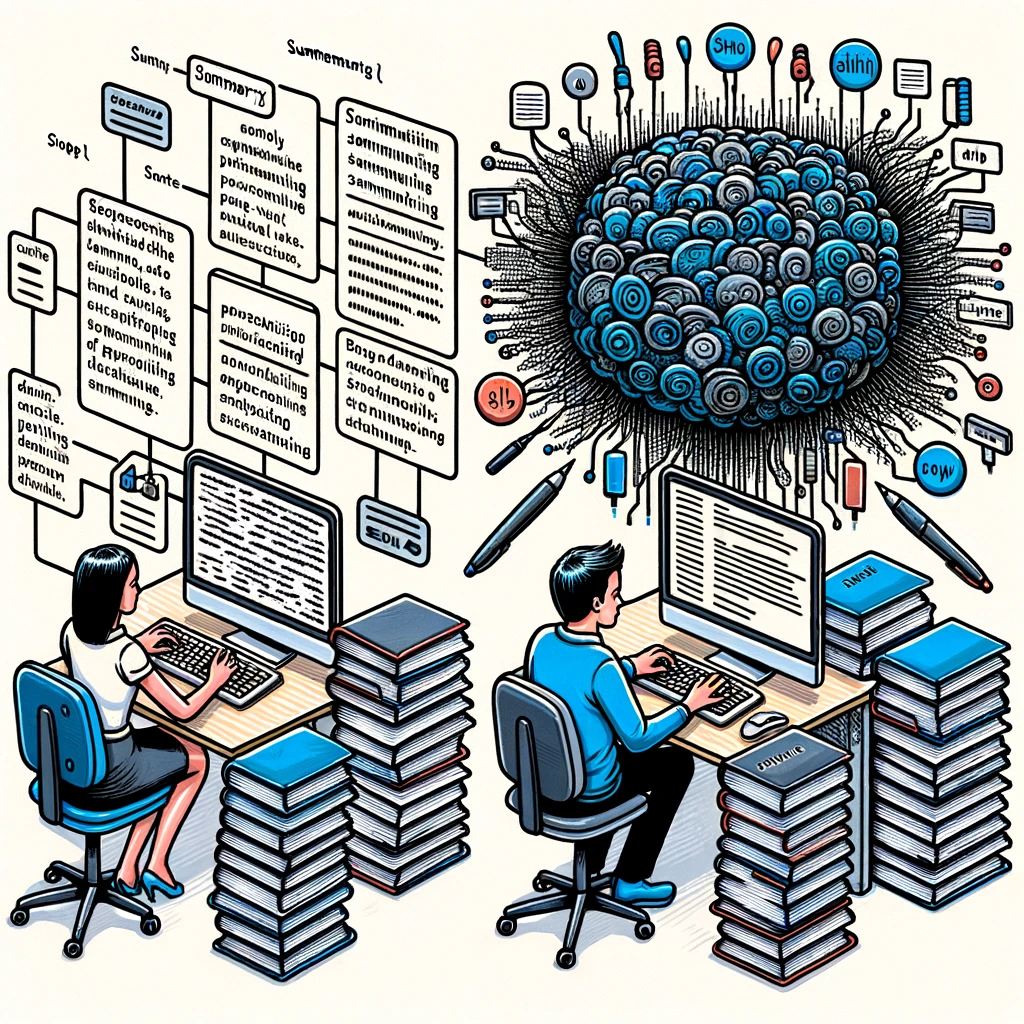
\includegraphics[width=0.5\textwidth]{../../img/programowanie ai vs klasyczne2.png}
                    \end{figure}                    
                    \end{itemize}
\end{frame}

\begin{frame}[fragile]
\frametitle{Przykład}
\begin{itemize}
\item Aby odpowiedzieć na te pytanie musimy zagłębić się nieco bardziej w sam proces programowania i zrozumieć czym różni się klasyczne programowanie od programowania sztucznej inteligencji. Najlepiej zrobić to na przykładzie.
\item Przyjmijmy, że naszym zadaniem jest napisanie programu komputerowego, który dla zadanego tekstu, np. artykułu prasowego (2-3 strony), będzie tworzył jego streszczenie (powiedzmy, max 10 zdań). 
\end{itemize}
\end{frame}

\begin{frame}[fragile]
\frametitle{Programowanie sztucznej inteligencji vs. programowanie klasyczne}
\begin{itemize}
\item \textbf{Klasyczne podejście do tego problemu} polega na tym, że programist(k)a najpierw sam(a) musi wymyślić jak taki problem rozwiązać (np. wytnij 3 pierwsze zdania ze wstępu artykułu i 2 ostatnie z zakończenia). Następnie programist(k)a zapisuje krok po kroku swój pomysł rozwiązania problemu w języku programowania i komputer go wykonuje.
\item \textbf{Programowanie sztucznej inteligencji} odwraca ten proces. Programist(k)a nie komunikuje komputerowi przepisu/algorytmu jak krok po kroku problem rozwiązać (przypomnijmy, w naszym przykładzie: jak na podstawie artykułu napisać jego streszczenie), ale \textbf{tworzy w samym komputerze środowisko/przestrzeń}, w której komputer na podstawie wielu przykładów artykułów prasowych i ich streszczeń sam taki przepis wymyśli. 
\end{itemize}
\end{frame}

\begin{frame}[fragile]
\frametitle{Sztuczne sieci neuronowe}
\begin{itemize}
\item Przestrzenią/środowiskiem, gdzie komputer samodzielnie szuka rozwiązania problemu są najczęściej \textbf{sztuczne sieci neuronowe}. Programist(k)a najpierw programuje jak taka sieć ma wyglądać, tzn., ile ma mieć neuronów, jaką ma mieć architekturę, czyli jak bardzo ma być złożona. Następnie określa długość procesu uczenia - w praktyce określa ile razy komputer ma “studiować” zgromadzone wcześniej przykłady artykułów i ich streszczeń. Choć może brzmieć to dość tajemniczo, to nie jest to bardzo skomplikowane.
\item Z racji na to inne podejście do programowania sztucznej inteligencji, raczej mówi się o \textbf{trenowaniu sztucznej inteligencji} niż o jej programowaniu. Nie zmienia to jednak faktu, że nadal jest to program komputerowy. 
\end{itemize}
\end{frame}

\begin{frame}[fragile]
\frametitle{Sztuczne sieci neuronowe}
\begin{itemize}
\item Podsumowując powiedzmy
	\begin{itemize}
	\item główną trudnością przy klasycznym programowaniu byłoby wymyślenie przez programist(k)ę jak utworzyć streszczenia z artykułów prasowych
	\item przy trenowaniu sztucznej inteligencji głównym problemem jest, po pierwsze, stworzenie pokaźnego materiału do uczenia komputera, nazywanego \textbf{zbiorem treningowym}, złożonego z artykułów prasowych i ich gotowych streszczeń i, po drugie, dobranie odpowiedniej \textbf{architektury sieci neuronowej} oraz \textbf{zdefiniowanie długości procesu uczenia}.
	\end{itemize}
\end{itemize}

\end{frame}

\section{OUTRO}

\begin{frame}[fragile]
\frametitle{Powiedzieliśmy, że...}
 \begin{itemize}
\item \textbf{Programowanie} to sposób komunikacji człowieka z komputerem, którego celem jest rozwiązanie jakiegoś problemu.
\item \textbf{Programist(k)a} to człowiek, który potrafi komunikację z komputerem skutecznie prowadzić. 
\item \textbf{Program komputerowy} to zbiór instrukcji które mówią komputerowi, co ma robić krok po kroku, zgodnie z intencją programisty lub programistki. 
\item \textbf{Inteligencja} to złożony zestaw różnych procesów myślowych, które umożliwiają przetwarzanie informacji, rozwiązywanie problemów, rozumienie emocji, podejmowanie decyzji i wykonywanie różnych działań. Nie ma jednej inteligencji, jest ich wiele! 
\end{itemize}
\end{frame}

\begin{frame}[fragile]
\frametitle{Powiedzieliśmy, że...}
\begin{itemize}
\item \textbf{Programy komputerowe nazwiemy inteligentnymi}, gdy automatyzują jakieś procesy myślowe standardowo wykonywane przez ludzi.
\item \textbf{Programowanie (trenowanie) sztucznej inteligencji} polega na tworzeniu w komputerze środowiska (najczęściej sztucznych sieci neuronowych), w  którym komputer na podstawie wielu przykładów, nazywanych zbiorem treningowym, sam wypracowuje rozwiązanie zadanego problemu. 
\end{itemize}
\end{frame}


\end{document}
    